\documentclass{article}
\usepackage{multicol}
\usepackage{xcolor}
\usepackage{graphicx}
\linespread{1.35}
\usepackage{amsmath}
\usepackage{color}
\usepackage{tikz}
\usetikzlibrary{arrows,automata}

\begin{document}

\begin{flushright}
 \texttt{Finite Automata} \hspace*{0.1cm}\textbf{$|$} \hspace*{0.1cm} \textbf{81}\hspace*{0.1cm}
\end{flushright}
\vspace*{1cm}

\begin{center}
\section{picture}
\includegraphics[width=8cm,height=5cm]{81.png}
\end{center}

\LARGE{\textbf{3.14 Minimization of Finite Automata}}

\vspace*{0.2cm}
\small{The language (regular expression) produced by a DFA is always unique. But the reverse, i.e., a language
produces a unique DFA, is not true. For this reason, there may be different DFAs in a given language.
By minimizing, we can get a minimized DFA with minimum number of states and transitions which
produces that particular language. The DFA determines how computers manipulate regular languages
(expressions). The DFA size determines the space/time efficiency. So, a DFA with minimized states
needs less time to manipulate a regular expression.

\hspace*{0.2cm} Before describing the process, we need to know the defi nitions of dead state, inaccessible state,
equivalent state, distinguishable state, and k-equivalence in relation with finite automata.}

\begin{itemize}
  \item \textbf{Dead State:} A state $q_i$ is called a dead state if $q_i$ is not a final state and for all the inputs to this
state, the transitions are confined to that state. In mathematical notation, we can denote $q_i \in  F$ and
$\delta(q_i, \Sigma) \rightarrow q_i$.
  \item \textbf{Inaccessible State:} The states which can never be reached from the initial state are called inaccessible
states.
\end{itemize}

\begin{center}
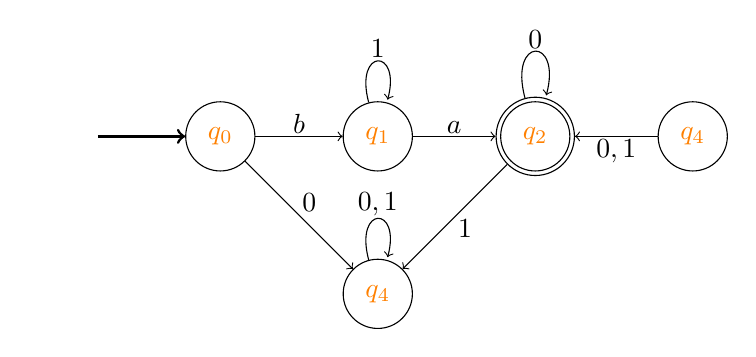
\begin{tikzpicture}[node distance = 2cm,auto,inner sep=1pt]
\node[state,draw=white,inner sep=0pt] (A) {$$};
\node[state,text=orange,draw=black] (B) [ right of = A]  {$q_0$};
\node[state,text=orange,draw=black] (C) [right of = B]  {$q_1$};
\node[state,text=orange,draw=black,inner sep=10pt] (D) [right of = C]  {$$};
\node[state,text=orange,draw=black] (E) [right of = C]  {$q_2$};
\node[state,text=orange,draw=black] (F) [ right of = D]  {$q_4$};
\node[state,text=orange,draw=black] (G) [below of = C]  {$q_4$};
\path (A) edge [->,line width=1pt,node distance = 0.1cm] node {$$} (B);
\path (B) edge [->] node {$b$} (C);
\path (C) edge [->] node {$a$} (D);
\path (C) edge [->,loop above] node {$1$} (C);
\path (D) edge [->,loop above] node {$0$} (D);
\path (F) edge [->] node {$0,1$} (D);
\path (D) edge [->] node {$1$} (G);
\path (B) edge [->] node {$0$} (G);
\path (G) edge [->,loop above] node {$0,1$} (G);
\end{tikzpicture}
\end{center}
\begin{center}
\textbf{Fig. 3.48}
\end{center}

Here, $q_d$ is a dead state and $q_a$ is an inaccessible state as shown in Fig. 3.48.

\begin{itemize}
  \item \textbf{Equivalent state:} Two states $q_i$ and $q_j$ of a finite automata M are called equivalent if both $\delta(q_i, x)$ and
$\delta(q_j, x)$ produce final states or both of them produce non-final states for all $x \varepsilon \Sigma*$. It is denoted by $q_i \equiv q_j$.
  \item \textbf{Distinguishable state:} Two states $q_i$ and $q_j$ of a finite automata M are called distinguishable if, for
a minimum length string x, for $\delta(q_i, x)$ and $\delta(q_j, x)$, one produces final state and another produces
non-final state or vice versa for all $x \varepsilon \Sigma*$.
\end{itemize}

\begin{flushleft}
    \textbf{82}\hspace*{0.1cm} \textbf{$|$} \hspace*{0.1cm} \texttt{Introduction to Automata Theory, Formal Languages and Computation}
  \end{flushleft}

\begin{itemize}
  \item \textbf{K-equivalent:} Two states $q_i$ and $q_j$ of a finite automata M are called k-equivalent $(k > = 0)$ if both
$\delta(q_i, x)$ and $\delta(q_j, x)$ produce final states or both of them produce non-final states for all $x \in \Sigma*$ of
length k or less.
\end{itemize}

\vspace*{0.3cm}

\LARGE{\textbf{3.14.1 Process of Minimizing}}

\vspace*{0.2cm}

\begin{itemize}
 \small{ \item All the states are ‘0’ equivalent. Mark this as $S_0$.
  \item Divide the set of states into two subsets: set of final states and set of non-final states. Mark this
as $S_1$.
  \item Apply all the inputs separately on the two subsets and find the next state combinations. If it happens
that, for applying input on one set of states, the next states belong to different subsets, then
separate the states which produce next states belonging to different subsets.
  \item Continue step $(3)$ for $n + 1$ times.
  \item If $S_n$ and $S_n + 1$ are the same, then stop and declare $S_n$ as an equivalent partition.
  \item Mark each subset of $S_n$ as a different state and construct the transitional table accordingly. This is
the minimum automata.}
\end{itemize}

Consider the following examples to make the minimization process clear.

\vspace*{0.3cm}
\fcolorbox{red}{blue}{\textbf{Example 3.25}}\hspace*{0.1cm} \texttt{Construct a minimum state automaton from the transitional table given below.}

\begin{center}
\section{picture}
\includegraphics[width=6cm,height=4cm]{82.png}
\end{center}

\emph{\textbf{Solution:}} In the finite automata, the states are $\{q_0, q_1, q_2, q_3, q_4, q_5\}$. Name this set as $S_0$.
\begin{center}
$S_0: \{q_0, q_1, q_2, q_3, q_4, q_5\}$
\end{center}

All of the states are 0 equivalents.\\
\hspace*{0.2cm} In the finite automata, there are two types of states: final state and non-final states. So, divide the set
of states into two parts, $Q_1$ and $Q_2$.\\

\begin{center}
$Q_1 = \{q_0, q_1, q_2\} Q_2 = \{q_3, q_4, q_5\}$

\vspace*{0.1cm}
\[
S_1: \{\{q_0, q_1, q_2\}, \{q_3, q_4, q_5\}\}
\]
\end{center}


\begin{flushright}
 \texttt{Finite Automata} \hspace*{0.1cm}\textbf{$|$} \hspace*{0.1cm} \textbf{83}\hspace*{0.1cm}
\end{flushright}

\vspace*{1cm}
The states belonging to the same subset are 1-equivalent because they are in the same set for string
length 1. The states belonging to different subsets are 1-distinguishable.\\
\hspace*{0.1cm} For input $0$ and $1$, $q_0$ goes to $q_1$ and $q_2$, respectively. Both of the states belong to the same subset. For
$q_1$ and $q_2$ with input $0$ and $1$, the next states are $q_2$, $q_3$ and $q_2$, $q_4$, respectively. For both of the states, for
input $0$, the next state belongs to one subset, and for input $1$, the next state belongs to another subset. So,
$q_0$ can be distinguished from $q_1$ and $q_2$.\\
\hspace*{0.1cm}The next states with input $0$ and $1$ for states $q_3$, $q_4$, and $q_5$ belong to the same subset. So, they cannot
be divided.

\vspace*{1cm}
\begin{center}
$S_2: \{\{q_0\}, \{q_1, q_2\}, \{q_3, q_4, q_5\}\}$
\end{center}

$q_0$ is the single state in the subset. So, it cannot be divided.\\
\hspace*{0.1cm} For states $q_1$ and $q_2$ with input 0 and 1, for both of the cases, one state belongs to one subset and
another state belongs to another subset. So, they cannot be divided.\\
\hspace*{0.1cm} The next states with input 0 and 1 for states q3, q4, and q5 belong to the same subset. So, they cannot
be divided.\\
\hspace*{0.1cm} So, in the next step,

\vspace*{1cm}
\begin{center}
$S_3: \{\{q_0\}, \{q_1, q_2\}, \{q_3, q_4, q_5\}\}$
\end{center}

$S_2$ and $S_3$ are equivalent.\\
As step $(n–1)$ and step n are the same, there is no need of further advancement.\\
In the minimized automata, the number of states is $3$.\\
The minimized finite automata is presented in tabular format as follows:

\begin{center}
\begin{tabular}{ccc}
 \hline

 \hline

 \hline

 \hline
 & \multicolumn{2}{c}{$Next State$}\\
 \cline{2-3}
 $State$ &  $I/P=0$ & $I/P=1$\\
\hline
 $\{q_0\}$           &   $\{q-1\}$           &  $\{q_2\}$          \\
 $\{q-1,q_2\}$       &   $\{q_2\}$           &  $\{q_3,q_4\}$      \\
 $\{q_3,q_4,q_5\}$   &   $\{q_3,q_4,q_5\}$   &  $\{q_3,q_4,q_5\}$  \\
 \hline

 \hline

 \hline

 \hline
\end{tabular}
\end{center}

But $\{q_1\}$, $\{q_2\}$, and $\{q_3, q_4\}$ do not exist under the column of present state. They are not states of the
minimized finite automata, but they are subset of the states. In the next state columns, by replacing the
subsets by proper state, the modified table becomes


\begin{center}
\begin{tabular}{ccc}
 \hline

 \hline

 \hline

 \hline
 & \multicolumn{2}{c}{$Next State$}\\
 \cline{2-3}
 $State$ &  $I/P=0$ & $I/P=1$\\
\hline
 $\{q_0\}$           &   $\{q-1,q_2\}$      &  $\{q-1,q_2\}$          \\
 $\{q-1,q_2\}$       &   $\{q-1,q_2\}$      &  $\{q_3,q_4,q_5\}$   \\
 $\{q_3,q_4,q_5\}$   &   $\{q_3,q_4,q_5\}$  &  $\{q_3,q_4,q_5\}$  \\
 \hline

 \hline

 \hline

 \hline
\end{tabular}
\end{center}


As $q_0$ is the beginning state of the original finite automata, $\{q_0\}$ will be the beginning state of minimized
finite automata. As $q_3$, $q_4$, and $q_5$ are the final states of the original finite automata, the set of the states
containing any of the states as element is final state. Here, all the states are contained in a single set
$\{q_3, q_4, q_5\}$ and, therefore, it is the final state. By replacing $\{q_0\}$ as $A$, $\{q_1, q_2\}$ as $B$, and $\{q_3, q_4, q_5\}$ as C,
the modified minimized finite automata becomes

\begin{flushleft}
    \textbf{84}\hspace*{0.1cm} \textbf{$|$} \hspace*{0.1cm} \texttt{Introduction to Automata Theory, Formal Languages and Computation}
  \end{flushleft}

\begin{center}
\section{picture}
\includegraphics[width=5cm,height=3cm]{84.png}
\end{center}

The transitional diagram of the minimized finite automata is given in Fig. 3.49.

\begin{center}
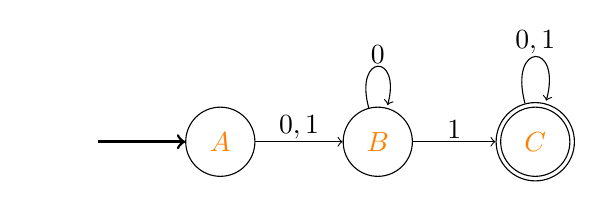
\begin{tikzpicture}[node distance = 2cm,auto,inner sep=1pt]
\node[state,draw=white,inner sep=0pt] (A) {$$};
\node[state,text=orange,draw=black] (B) [ right of = A]  {$A$};
\node[state,text=orange,draw=black] (C) [right of = B]  {$B$};
\node[state,text=orange,draw=black,inner sep=10pt] (D) [right of = C]  {$$};
\node[state,text=orange,draw=black] (E) [right of = C]  {$C$};

\path (A) edge [->,line width=1pt,node distance = 0.1cm] node {$$} (B);
\path (B) edge [->] node {$0,1$} (C);
\path (C) edge [->] node {$1$} (D);
\path (C) edge [->,loop above] node {$0$} (C);
\path (D) edge [->,loop above] node {$0,1$} (D);

\end{tikzpicture}
\end{center}
\begin{center}
\textbf{Fig. 3.49}
\end{center}

\fcolorbox{red}{blue}{\textbf{Example 3.26}}\hspace*{0.1cm} \texttt{Construct a minimum state automaton from the following transitional table.}

\begin{center}
\begin{tabular}{ccc}
 \hline

 \hline

 \hline

 \hline
 & \multicolumn{2}{c}{$Next State$}\\
 \cline{2-3}
 $Present State$ &  $I/P=0$ & $I/P=1$\\
\hline
 $A$    &    $F$    &   $B$  \\
 $B$    &    $C$    &   $G$  \\
 $C$    &    $C$    &   $A$  \\
 $D$    &    $G$    &   $C$  \\
 $E$    &    $F$    &   $H$  \\
 $F$    &    $G$    &   $C$  \\
 $G$    &    $E$    &   $G$  \\
 $H$    &    $C$    &   $G$  \\
 \hline

 \hline

 \hline

 \hline
\end{tabular}
\end{center}
A is initial state and C is final state

\emph{\textbf{Solution:}} In the Finite automata, the states are $\{A, B, C, D, E, F, G, H\}$. Name this set as $S_0$.\\

\begin{center}
$S_0: \{A, B, C, D, E, F, G, H\}$
\end{center}

\vspace*{0.1cm}
\hspace*{0.2cm} All of the states are 0 equivalents.\\
In the finite automata, there are two types of states: final state and non-final state. The set of states is
divided into two parts, namely, $Q_1$ and $Q_2$.

\begin{center}
  $Q_1 = \{C\} Q_2 = \{A, B, D, E, F, G, H\}$ \\
  $S_1: \{\{C\} \{A, B, D, E, F, G, H\}\}$
\end{center}

\small{
The states belonging to the same subset are 1-equivalent because they are in the same set for string
length 1. The states belonging to different subsets are 1-distinguishable.\\
\hspace*{0.2cm} C is a single state, and so it cannot be divided. Among the states $\{A, B, D, E, F, G, H\}$ for $\{B, D, F, H\}$,
for an input of either 0 or 1, the next state belongs to $\{C\}$ which is a different subset (from B with input 0
goes to C, from D with input 1 goes to C, from F with input 1 goes to C, and from H with input 0 goes to C).}

\end{document}